% Observed saved-data coverage only; no post-removal accuracy claim.
\subsection{Training-only selection and common controls}
\label{sec:expert-memory-study}

We compare state-balanced retention, pooled labelled-token frequency and
the original fixed random control at 75\% retained expert identities per
routed layer. The layer quotas are 24, 96, 192, 192, 96, 48 and 96 experts
for GPT-OSS, Nemotron, Qwen3.5, Qwen3.6, Gemma, GLM and Qwen3-30B,
respectively. These are selections evaluated on saved native traces;
no expert is removed during this analysis. Serialized checkpoint bytes
and actual GPU residence are separate quantities.

Five common retrospective folds group the 1,547 historical questions into
1,486 duplicate families. A family has total weight one, shared equally among
its member questions. For class $c$, layer $\ell$ and expert $e$, first average
selected-slot counts over questions within family $f$, giving $C_{fc\ell e}$.
The state-balanced score is
\begin{equation}
 s^{\mathrm{bal}}_{\ell e}
 =\frac{1}{|\mathcal C|}\sum_{c\in\mathcal C}
   \frac{1}{|\mathcal F_c|}\sum_{f\in\mathcal F_c}
   \frac{C_{fc\ell e}}{\sum_j C_{fc\ell j}},
\end{equation}
where $\mathcal F_c$ contains training families with observed class $c$.
Every class requires training support. The frequency control pools the same
family-weighted labelled counts, proportional to their observed token mass:
\begin{equation}
 s^{\mathrm{freq}}_{\ell e}
 =\frac{\sum_{f,c}C_{fc\ell e}}{\sum_{f,c,j}C_{fc\ell j}}.
\end{equation}

Both learned methods use training families only, identical layer/group
quotas and original expert ID to break ties. Neither uses correctness to
rank experts. Random priorities use seed 20261008 and fix one set per
model; the comparison is conditional on those sets. The frequency arm
uses labelled tokens, so it is not a comparison against every conventional
all-token or output-aware pruning criterion.

For each held-out fold and class, coverage is the retained fraction of
family-weighted native selected slots at each layer, averaged equally
over routed layers. The primary descriptive summary takes the minimum
over all seven classes. Every displayed fold has complete class coverage.
It measures which original selections a keep-set contains, rather than
what the model would do after rerouting.

\subsection{Observed model-dependent coverage}

The complete five-fold analysis covers all seven models
(Figure~\ref{fig:expert-memory-heldout}). State balancing has higher minimum
class coverage than pooled labelled frequency in every fold for GPT-OSS,
Nemotron, Gemma, GLM and Qwen3-30B. Pooled labelled frequency is higher in
every fold for Qwen3.5 and Qwen3.6. The arithmetic mean paired differences
across folds are $+1.77$, $+4.58$, $+0.21$, $+2.79$ and $+0.59$ percentage
points for GPT-OSS, Nemotron, Gemma, GLM and Qwen3-30B, respectively. They
are $-1.35$ for Qwen3.5 and $-0.55$ for Qwen3.6. The fixed random masks have
minimum class coverage between 73.4\% and 77.2\% across the model/fold
cells. All five folds are shown, including the two models favoring
frequency. Their spread describes partition stability, not a confidence
interval; folds with overlapping training data are not independent
replications.

\begin{figure}[t]
\centering
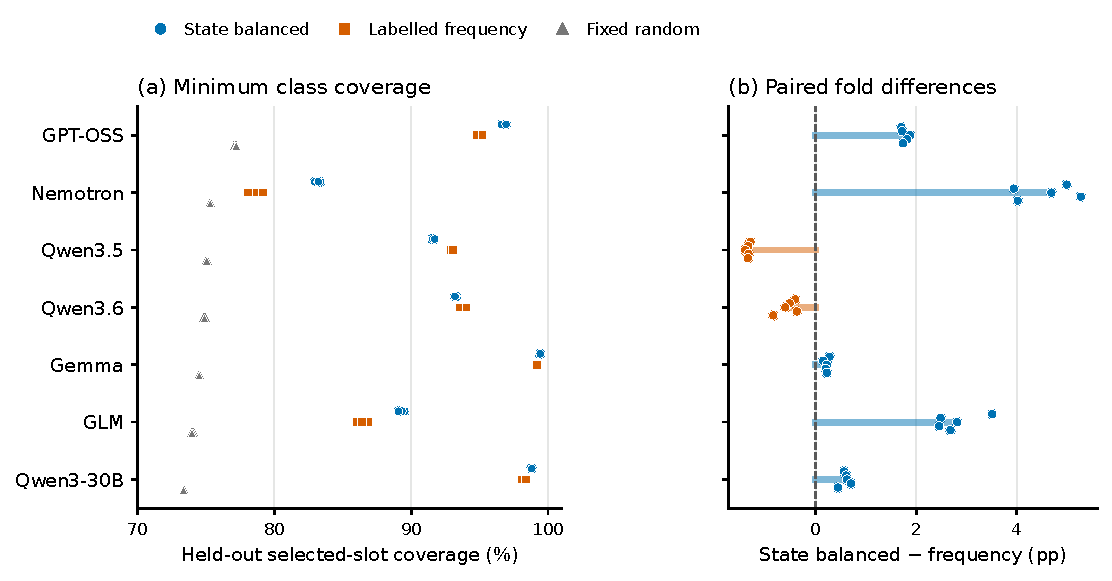
\includegraphics[width=\linewidth]{generated/best_results_20261009/heldout_retention.pdf}
\caption{Minimum held-out reasoning-class coverage at 75\% expert retention.
(a) All five common duplicate-family folds for each selection method;
horizontal lines connect the fold extrema. (b) All five paired
state-balanced-minus-frequency differences; bars end at their descriptive
fold mean. Coverage averages layers within class before taking the minimum.
The comparison uses training-only selection and identical quotas. Neither
fold ranges nor mean bars are inferential intervals.}
\label{fig:expert-memory-heldout}
\end{figure}

The comparison shows that balancing labelled states can improve the
least-covered class at a fixed identity budget, but the direction and
magnitude depend on the model. Near-complete coverage in Gemma and
Qwen3-30B also leaves little room for a large coverage improvement.
These observations establish neither accuracy retention after physical
removal nor a realized GPU-memory saving. Missing and unlabelled tokens
remain outside this class-conditioned endpoint.
